\documentclass{standalone}
\usepackage{tikz}
\usetikzlibrary{patterns, positioning}


\begin{document}
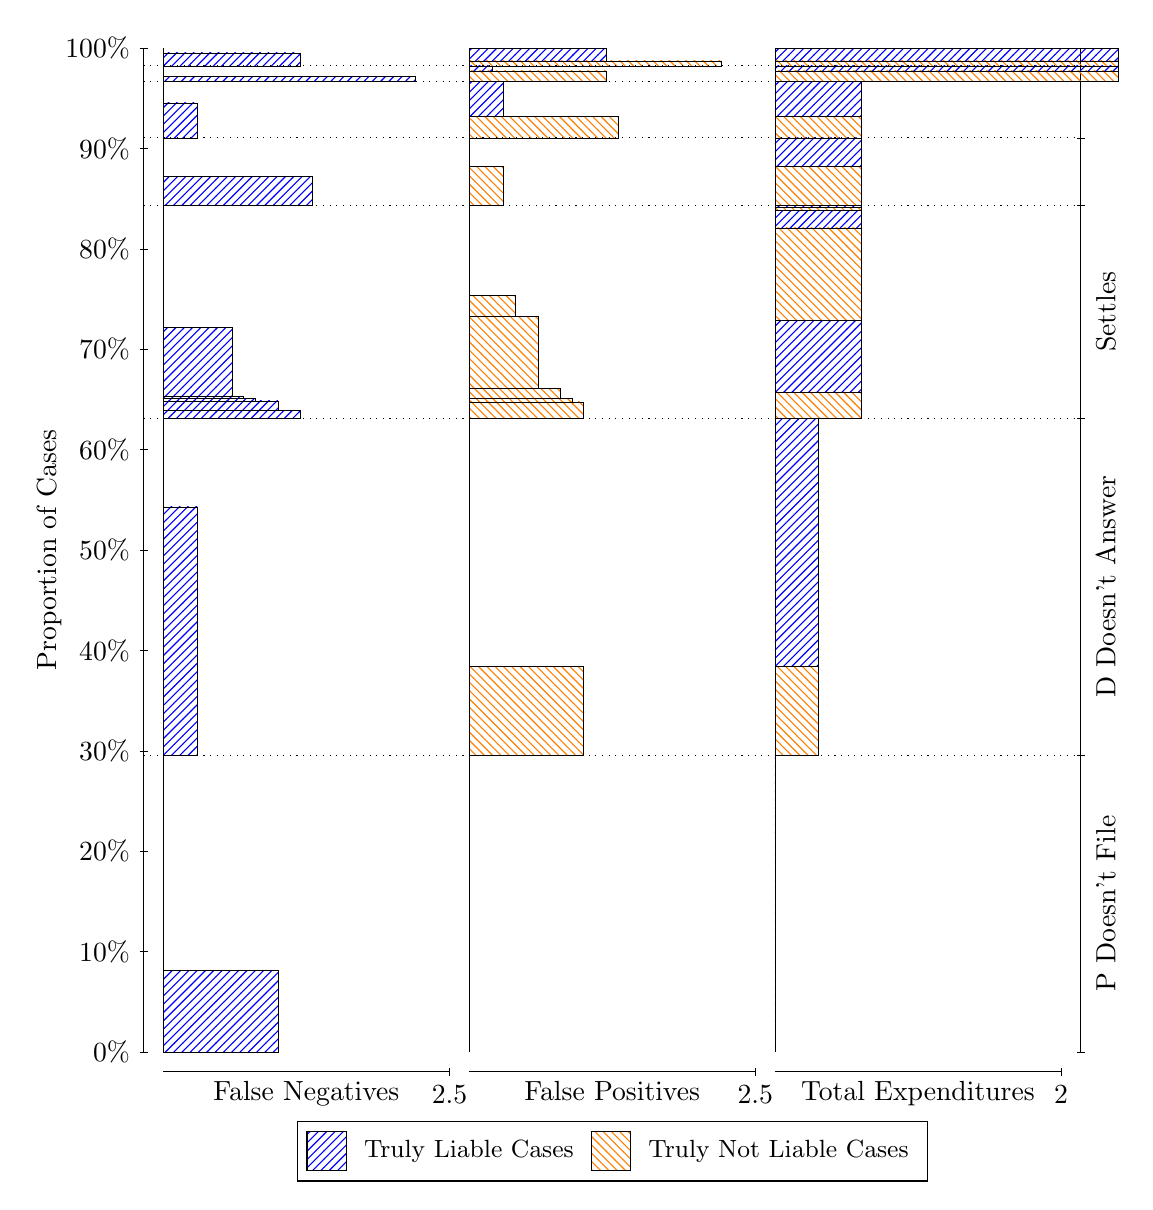
\begin{tikzpicture}
\draw[black, very thin] (1.5,1.75) -- (1.5,14.5);
\node[rotate=90, text=black, anchor=center] at (0.3, 8.125) {Proportion of Cases};
\draw[black, very thin] (1.45,1.75) -- (1.55,1.75);
\node[text=black, anchor=east] at (1.45, 1.75) {0\%};
\draw[black, very thin] (1.45,3.025) -- (1.55,3.025);
\node[text=black, anchor=east] at (1.45, 3.025) {10\%};
\draw[black, very thin] (1.45,4.3) -- (1.55,4.3);
\node[text=black, anchor=east] at (1.45, 4.3) {20\%};
\draw[black, very thin] (1.45,5.575) -- (1.55,5.575);
\node[text=black, anchor=east] at (1.45, 5.575) {30\%};
\draw[black, very thin] (1.45,6.85) -- (1.55,6.85);
\node[text=black, anchor=east] at (1.45, 6.85) {40\%};
\draw[black, very thin] (1.45,8.125) -- (1.55,8.125);
\node[text=black, anchor=east] at (1.45, 8.125) {50\%};
\draw[black, very thin] (1.45,9.4) -- (1.55,9.4);
\node[text=black, anchor=east] at (1.45, 9.4) {60\%};
\draw[black, very thin] (1.45,10.675) -- (1.55,10.675);
\node[text=black, anchor=east] at (1.45, 10.675) {70\%};
\draw[black, very thin] (1.45,11.95) -- (1.55,11.95);
\node[text=black, anchor=east] at (1.45, 11.95) {80\%};
\draw[black, very thin] (1.45,13.225) -- (1.55,13.225);
\node[text=black, anchor=east] at (1.45, 13.225) {90\%};
\draw[black, very thin] (1.45,14.5) -- (1.55,14.5);
\node[text=black, anchor=east] at (1.45, 14.5) {100\%};

\draw[black, very thin] (13.4,1.75) -- (13.4,14.5);
\draw[black, very thin] (13.35,1.75) -- (13.45,1.75);
\node[anchor=west] at (13.35, 1.75) {};
\draw[black, very thin] (13.35,5.5194) -- (13.45,5.5194);
\node[anchor=west] at (13.35, 5.5194) {};
\draw[black, very thin] (13.35,9.7996) -- (13.45,9.7996);
\node[anchor=west] at (13.35, 9.7996) {};
\draw[black, very thin] (13.35,12.504) -- (13.45,12.504);
\node[anchor=west] at (13.35, 12.504) {};
\draw[black, very thin] (13.35,13.359) -- (13.45,13.359);
\node[anchor=west] at (13.35, 13.359) {};
\draw[black, very thin] (13.35,14.08) -- (13.45,14.08);
\node[anchor=west] at (13.35, 14.08) {};
\draw[black, very thin] (13.35,14.274) -- (13.45,14.274);
\node[anchor=west] at (13.35, 14.274) {};
\draw[black, very thin] (13.35,14.5) -- (13.45,14.5);
\node[anchor=west] at (13.35, 14.5) {};

\draw[black, very thin, pattern color=blue, pattern=north east lines] (1.75,1.75) rectangle (3.2033,2.7884);
\draw[black, very thin, pattern color=orange, pattern=north west lines] (1.75,2.7884) rectangle (1.75,5.5194);
\draw[black, very thin, pattern color=blue, pattern=north east lines] (1.75,5.5194) rectangle (2.186,8.6731);
\draw[black, very thin, pattern color=orange, pattern=north west lines] (1.75,8.6731) rectangle (1.75,9.7996);
\draw[black, very thin, pattern color=blue, pattern=north east lines] (1.75,9.7996) rectangle (3.494,9.9002);
\draw[black, very thin, pattern color=blue, pattern=north east lines] (1.75,9.9002) rectangle (3.2033,10.018);
\draw[black, very thin, pattern color=blue, pattern=north east lines] (1.75,10.018) rectangle (2.9127,10.048);
\draw[black, very thin, pattern color=blue, pattern=north east lines] (1.75,10.048) rectangle (2.7673,10.073);
\draw[black, very thin, pattern color=blue, pattern=north east lines] (1.75,10.073) rectangle (2.622,10.948);
\draw[black, very thin, pattern color=orange, pattern=north west lines] (1.75,10.948) rectangle (1.75,12.504);
\draw[black, very thin, pattern color=blue, pattern=north east lines] (1.75,12.504) rectangle (3.6393,12.868);
\draw[black, very thin, pattern color=orange, pattern=north west lines] (1.75,12.868) rectangle (1.75,13.359);
\draw[black, very thin, pattern color=blue, pattern=north east lines] (1.75,13.359) rectangle (2.186,13.803);
\draw[black, very thin, pattern color=orange, pattern=north west lines] (1.75,13.803) rectangle (1.75,14.08);
\draw[black, very thin, pattern color=blue, pattern=north east lines] (1.75,14.08) rectangle (4.9473,14.143);
\draw[black, very thin, pattern color=orange, pattern=north west lines] (1.75,14.143) rectangle (1.75,14.274);
\draw[black, very thin, pattern color=blue, pattern=north east lines] (1.75,14.274) rectangle (3.494,14.437);
\draw[black, very thin, pattern color=orange, pattern=north west lines] (1.75,14.437) rectangle (1.75,14.5);
\draw[black, very thin, pattern color=orange, pattern=north west lines] (5.6333,1.75) rectangle (5.6333,4.4811);
\draw[black, very thin, pattern color=blue, pattern=north east lines] (5.6333,4.4811) rectangle (5.6333,5.5194);
\draw[black, very thin, pattern color=orange, pattern=north west lines] (5.6333,5.5194) rectangle (7.0867,6.646);
\draw[black, very thin, pattern color=blue, pattern=north east lines] (5.6333,6.646) rectangle (5.6333,9.7996);
\draw[black, very thin, pattern color=orange, pattern=north west lines] (5.6333,9.7996) rectangle (7.0867,10.007);
\draw[black, very thin, pattern color=orange, pattern=north west lines] (5.6333,10.007) rectangle (6.9413,10.053);
\draw[black, very thin, pattern color=orange, pattern=north west lines] (5.6333,10.053) rectangle (6.796,10.177);
\draw[black, very thin, pattern color=orange, pattern=north west lines] (5.6333,10.177) rectangle (6.5053,11.088);
\draw[black, very thin, pattern color=orange, pattern=north west lines] (5.6333,11.088) rectangle (6.2147,11.355);
\draw[black, very thin, pattern color=blue, pattern=north east lines] (5.6333,11.355) rectangle (5.6333,12.504);
\draw[black, very thin, pattern color=orange, pattern=north west lines] (5.6333,12.504) rectangle (6.0693,12.995);
\draw[black, very thin, pattern color=blue, pattern=north east lines] (5.6333,12.995) rectangle (5.6333,13.359);
\draw[black, very thin, pattern color=orange, pattern=north west lines] (5.6333,13.359) rectangle (7.5227,13.636);
\draw[black, very thin, pattern color=blue, pattern=north east lines] (5.6333,13.636) rectangle (6.0693,14.08);
\draw[black, very thin, pattern color=orange, pattern=north west lines] (5.6333,14.08) rectangle (7.3773,14.211);
\draw[black, very thin, pattern color=blue, pattern=north east lines] (5.6333,14.211) rectangle (5.924,14.274);
\draw[black, very thin, pattern color=orange, pattern=north west lines] (5.6333,14.274) rectangle (8.8307,14.337);
\draw[black, very thin, pattern color=blue, pattern=north east lines] (5.6333,14.337) rectangle (7.3773,14.5);
\draw[black, very thin, pattern color=orange, pattern=north west lines] (9.5167,1.75) rectangle (9.5167,4.4811);
\draw[black, very thin, pattern color=blue, pattern=north east lines] (9.5167,4.4811) rectangle (9.5167,5.5194);
\draw[black, very thin, pattern color=orange, pattern=north west lines] (9.5167,5.5194) rectangle (10.062,6.646);
\draw[black, very thin, pattern color=blue, pattern=north east lines] (9.5167,6.646) rectangle (10.062,9.7996);
\draw[black, very thin, pattern color=orange, pattern=north west lines] (9.5167,9.7996) rectangle (10.607,10.132);
\draw[black, very thin, pattern color=blue, pattern=north east lines] (9.5167,10.132) rectangle (10.607,11.037);
\draw[black, very thin, pattern color=orange, pattern=north west lines] (9.5167,11.037) rectangle (10.607,12.215);
\draw[black, very thin, pattern color=blue, pattern=north east lines] (9.5167,12.215) rectangle (10.607,12.434);
\draw[black, very thin, pattern color=orange, pattern=north west lines] (9.5167,12.434) rectangle (10.607,12.479);
\draw[black, very thin, pattern color=blue, pattern=north east lines] (9.5167,12.479) rectangle (10.607,12.504);
\draw[black, very thin, pattern color=orange, pattern=north west lines] (9.5167,12.504) rectangle (10.607,12.995);
\draw[black, very thin, pattern color=blue, pattern=north east lines] (9.5167,12.995) rectangle (10.607,13.359);
\draw[black, very thin, pattern color=orange, pattern=north west lines] (9.5167,13.359) rectangle (10.607,13.636);
\draw[black, very thin, pattern color=blue, pattern=north east lines] (9.5167,13.636) rectangle (10.607,14.08);
\draw[black, very thin, pattern color=orange, pattern=north west lines] (9.5167,14.08) rectangle (13.877,14.211);
\draw[black, very thin, pattern color=blue, pattern=north east lines] (9.5167,14.211) rectangle (13.877,14.274);
\draw[black, very thin, pattern color=orange, pattern=north west lines] (9.5167,14.274) rectangle (13.877,14.337);
\draw[black, very thin, pattern color=blue, pattern=north east lines] (9.5167,14.337) rectangle (13.877,14.5);
\draw[black, dotted] (1.5,5.5194) -- (13.4,5.5194);
\draw[black, dotted] (1.5,9.7996) -- (13.4,9.7996);
\draw[black, dotted] (1.5,12.504) -- (13.4,12.504);
\draw[black, dotted] (1.5,13.359) -- (13.4,13.359);
\draw[black, dotted] (1.5,14.08) -- (13.4,14.08);
\draw[black, dotted] (1.5,14.274) -- (13.4,14.274);
\draw[black, very thin] (1.75,1.5) -- (5.3833,1.5);
\node[text=black, anchor=north] at (3.5667, 1.5) {False Negatives};
\draw[black, very thin] (5.3833,1.45) -- (5.3833,1.55);
\node[text=black, anchor=north] at (5.3833, 1.45) {2.5};

\draw[black, very thin] (5.6333,1.5) -- (9.2667,1.5);
\node[text=black, anchor=north] at (7.45, 1.5) {False Positives};
\draw[black, very thin] (9.2667,1.45) -- (9.2667,1.55);
\node[text=black, anchor=north] at (9.2667, 1.45) {2.5};

\draw[black, very thin] (9.5167,1.5) -- (13.15,1.5);
\node[text=black, anchor=north] at (11.333, 1.5) {Total Expenditures};
\draw[black, very thin] (13.15,1.45) -- (13.15,1.55);
\node[text=black, anchor=north] at (13.15, 1.45) {2};

\node[text=black, centered, rotate=90] at (13.72, 3.6347) {P Doesn't File};
\node[text=black, centered, rotate=90] at (13.72, 7.6595) {D Doesn't Answer};
\node[text=black, centered, rotate=90] at (13.72, 11.152) {Settles};





\draw (7.449999999999999,1.5) node[draw=none] (baseCoordinate) {};
\begin{scope}[align=center]
        \matrix[scale=0.5, draw=black, below=0.5cm of baseCoordinate, nodes={draw}, column sep=0.1cm]{
            \node[rectangle, draw, minimum width=0.5cm, minimum height=0.5cm, pattern color=blue, pattern=north east lines] {}; &
            \node[draw=none, font=\small, text=black] (B) {Truly Liable Cases}; &
            \node[rectangle, draw, minimum width=0.5cm, minimum height=0.5cm, pattern color=orange, pattern=north west lines] {}; &
            \node[draw=none, font=\small, text=black] (B) {Truly Not Liable Cases}; \\
            };
\end{scope}

\end{tikzpicture}
\end{document}